\chapter{Implémentation}

Pour mettre en place cette méthode, nous avons développé une paire client-serveur SPA en langage C.

La topologie utilisée lors du développement et des tests est un réseau de 4 machines virtuelles : 

\begin{figure}[h]

\centerline{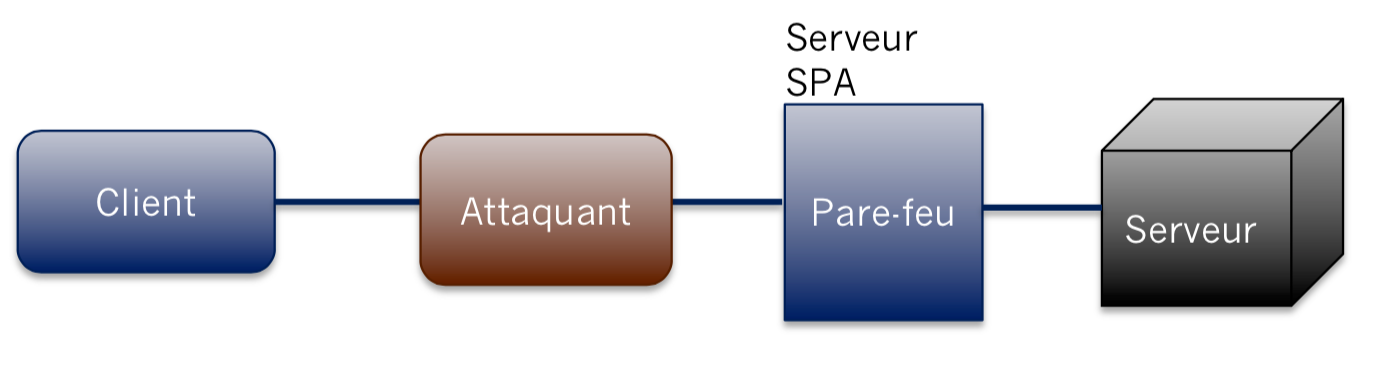
\includegraphics[scale=0.5]{topo_imple}}
\caption{Topologie du réseau de machines virtuelles}

\end{figure}
Nous avons ainsi fait appel à diverses librairies dont nous allons détailler l'intérêt.

\subsection{Libnet}
Dans un premier temps, nous avons eu besoin d'envoyer un paquet depuis le client vers le serveur, pour cela nous avons utilisé la librairie \emph{Libnet} qui nous a permis de mettre en place une socket RAW, de créer l'encapsulation IP, UDP et de placer les données à envoyer.

\subsection{Open SSL}
Afin d'authentifier cette demande, nous avons utilisé la librairie \emph{OpenSSL} possédant une documentation complète (voir bibliographie).
Les HMAC Based OTP, elle aussi, sont gérés grâce à la librairie \emph{OpenSSL}. Plus précisément, nous avons utilisé la fonction de calcul \emph{HMAC} qu'elle contient.

\subsection{Libpcap}
Pour récupérer ce paquet depuis le serveur, nous avons utilisé la librairie \emph{libpcap} qui nous a permis de filtrer les paquets afin de récupérer les \emph{SPA}. Nous avons pu différencier ces paquets grâce au fait qu'ils ont pour destination un port unique du pare-feu. Nous traitons ensuite ces requêtes une par une.

\subsection{Time.h}
Pour assurer une bonne gestion de l'horodatage aux client et au serveur SPA, nous avons utilisé la bibliothèque time.h
 afin de s'assurer que le temps utilisés ne patissent pas de problème de faisseaux horaires.

\subsection{LibXML2}

Enfin, nous avons, à l'aide de la librairie \emph{LibXML2}, enregistré les informations nécessaires à l'utilisation de HOTP dans un fichier \emph{XML} (au niveau client et serveur).
Ce fichier contient :
\begin{itemize}
\item \textbf{Au niveau du serveur SPA} ,une entrée par client authentifié. Dans cette entrée sont stockés la graine (secret partagé), le compteur et un identifiant (ici une adresse IP) permettant au serveur de différencier ses clients.
\item \textbf{Au niveau du client}, une seule entrée contenant le secret partagé et un compteur ayant, au temps \emph{t}, la même valeur pour le client et le serveur.
\end{itemize}

\subsection{Structure de connections actives}

Contrairement au fichier XML, nous souhaitons que le serveur garde en mémoire les connections actives. Nous utilisons donc une structure qui contient la liste des clients authentifié possédant en même temps une autorisation de communication particulière avec le serveur applicatif. Nous avons ainsi implémenter une liste chainée contenant, dans chaque cellule, des informations sur la connexion et sur le client qui en est à l'origine tout en permettant d'ajouter, de modifier ou de supprimer une entrée.
